% question 4
\section{Question 4}
Figure \ref{fig:q4} describes the block diagram for robot end-effector position control. The sensor block is formed by an encoder and forward kinematics. The encoder measures joint velocity and position, and forward kinematics relates joint configuration with end-effector position and orientation. Therefore, sensor block is one of the most important due to providing the feedback signal to the close-loop system.

\begin{figure}[h!]
	\centering
	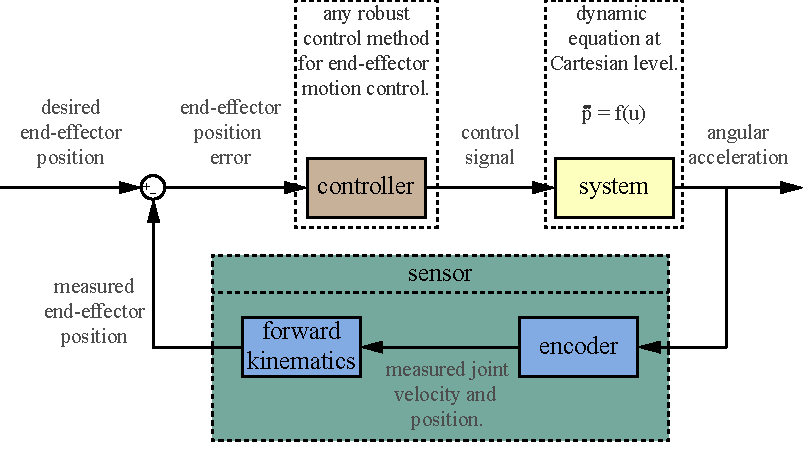
\includegraphics{q4.pdf}
	\caption{Block diagram for robot end-effector position control.}
	\label{fig:q4}
\end{figure}